In this chapter we go into detail about how the DSMC model is implemented in C{}\verb!++!. We assume that the reader is familiar with the programming language. Instead of going through all the classes and their relations, we follow the timeline of a simulation, going from the initialization of the system to how the timestep is computed. For convenience, an UML diagram is shown in figure \ref{fig:dsmc_uml_diagram}.
\begin{figure}[h]
\begin{center}
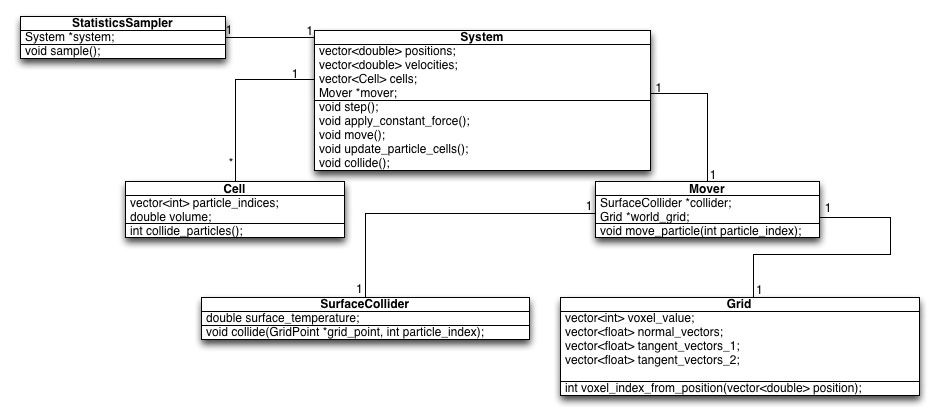
\includegraphics[width=0.9\textwidth, trim=0cm 0cm 0cm 0cm, clip]{DSMC/figures/dsmcuml.png}
\end{center}
\caption{A UML-diagram showing how the classes in the DSMC program are related to each other.}
\label{fig:dsmc_uml_diagram}
\end{figure}
\\
The first step of the full program is to create the geometry we want the particles to be confined by. We explain how that is done in section \ref{sec:dsmc_complex_geometries}. Then, we can initialize a system by adding particles randomly inside the geometry. Their velocities should be Maxwell-Boltzmann distributed, as described in section \ref{eq:maxwell_boltzmann_vector_probability}. The initialiation process is explained in section \ref{sec:dsmc_implementation_initialization} before we are ready to perform the timesteps. A timestep is divided into four stages. These stages are
\begin{itemize}
    \item accelerate particles to induce flow,
    \item move particles and perform surface interactions,
    \item update collision cells,
    \item perform collisions between particles,
\end{itemize}
which all are discussed in section \ref{sec:dsmc_implementation_timestep}. This is everything we need to run a DSMC program in \textit{any} geometry we want. The only thing left to explain is how we have parallelized the code, allowing it to run on many processors on a supercomputer. This final piece is explained in section \ref{sec:dmsc_parallelization}. 